% Options for packages loaded elsewhere
\PassOptionsToPackage{unicode}{hyperref}
\PassOptionsToPackage{hyphens}{url}
\PassOptionsToPackage{dvipsnames,svgnames,x11names}{xcolor}
%
\documentclass[
  9pt,
  a4paper,
  DIV=11]{scrreprt}

\usepackage{amsmath,amssymb}
\usepackage{iftex}
\ifPDFTeX
  \usepackage[T1]{fontenc}
  \usepackage[utf8]{inputenc}
  \usepackage{textcomp} % provide euro and other symbols
\else % if luatex or xetex
  \usepackage{unicode-math}
  \defaultfontfeatures{Scale=MatchLowercase}
  \defaultfontfeatures[\rmfamily]{Ligatures=TeX,Scale=1}
\fi
\usepackage{lmodern}
\ifPDFTeX\else  
    % xetex/luatex font selection
\fi
% Use upquote if available, for straight quotes in verbatim environments
\IfFileExists{upquote.sty}{\usepackage{upquote}}{}
\IfFileExists{microtype.sty}{% use microtype if available
  \usepackage[]{microtype}
  \UseMicrotypeSet[protrusion]{basicmath} % disable protrusion for tt fonts
}{}
\makeatletter
\@ifundefined{KOMAClassName}{% if non-KOMA class
  \IfFileExists{parskip.sty}{%
    \usepackage{parskip}
  }{% else
    \setlength{\parindent}{0pt}
    \setlength{\parskip}{6pt plus 2pt minus 1pt}}
}{% if KOMA class
  \KOMAoptions{parskip=half}}
\makeatother
\usepackage{xcolor}
\setlength{\emergencystretch}{3em} % prevent overfull lines
\setcounter{secnumdepth}{3}
% Make \paragraph and \subparagraph free-standing
\ifx\paragraph\undefined\else
  \let\oldparagraph\paragraph
  \renewcommand{\paragraph}[1]{\oldparagraph{#1}\mbox{}}
\fi
\ifx\subparagraph\undefined\else
  \let\oldsubparagraph\subparagraph
  \renewcommand{\subparagraph}[1]{\oldsubparagraph{#1}\mbox{}}
\fi


\providecommand{\tightlist}{%
  \setlength{\itemsep}{0pt}\setlength{\parskip}{0pt}}\usepackage{longtable,booktabs,array}
\usepackage{calc} % for calculating minipage widths
% Correct order of tables after \paragraph or \subparagraph
\usepackage{etoolbox}
\makeatletter
\patchcmd\longtable{\par}{\if@noskipsec\mbox{}\fi\par}{}{}
\makeatother
% Allow footnotes in longtable head/foot
\IfFileExists{footnotehyper.sty}{\usepackage{footnotehyper}}{\usepackage{footnote}}
\makesavenoteenv{longtable}
\usepackage{graphicx}
\makeatletter
\def\maxwidth{\ifdim\Gin@nat@width>\linewidth\linewidth\else\Gin@nat@width\fi}
\def\maxheight{\ifdim\Gin@nat@height>\textheight\textheight\else\Gin@nat@height\fi}
\makeatother
% Scale images if necessary, so that they will not overflow the page
% margins by default, and it is still possible to overwrite the defaults
% using explicit options in \includegraphics[width, height, ...]{}
\setkeys{Gin}{width=\maxwidth,height=\maxheight,keepaspectratio}
% Set default figure placement to htbp
\makeatletter
\def\fps@figure{htbp}
\makeatother
% definitions for citeproc citations
\NewDocumentCommand\citeproctext{}{}
\NewDocumentCommand\citeproc{mm}{%
  \begingroup\def\citeproctext{#2}\cite{#1}\endgroup}
\makeatletter
 % allow citations to break across lines
 \let\@cite@ofmt\@firstofone
 % avoid brackets around text for \cite:
 \def\@biblabel#1{}
 \def\@cite#1#2{{#1\if@tempswa , #2\fi}}
\makeatother
\newlength{\cslhangindent}
\setlength{\cslhangindent}{1.5em}
\newlength{\csllabelwidth}
\setlength{\csllabelwidth}{3em}
\newenvironment{CSLReferences}[2] % #1 hanging-indent, #2 entry-spacing
 {\begin{list}{}{%
  \setlength{\itemindent}{0pt}
  \setlength{\leftmargin}{0pt}
  \setlength{\parsep}{0pt}
  % turn on hanging indent if param 1 is 1
  \ifodd #1
   \setlength{\leftmargin}{\cslhangindent}
   \setlength{\itemindent}{-1\cslhangindent}
  \fi
  % set entry spacing
  \setlength{\itemsep}{#2\baselineskip}}}
 {\end{list}}
\usepackage{calc}
\newcommand{\CSLBlock}[1]{\hfill\break\parbox[t]{\linewidth}{\strut\ignorespaces#1\strut}}
\newcommand{\CSLLeftMargin}[1]{\parbox[t]{\csllabelwidth}{\strut#1\strut}}
\newcommand{\CSLRightInline}[1]{\parbox[t]{\linewidth - \csllabelwidth}{\strut#1\strut}}
\newcommand{\CSLIndent}[1]{\hspace{\cslhangindent}#1}

\makeatletter
\@ifpackageloaded{tcolorbox}{}{\usepackage[skins,breakable]{tcolorbox}}
\@ifpackageloaded{fontawesome5}{}{\usepackage{fontawesome5}}
\definecolor{quarto-callout-color}{HTML}{909090}
\definecolor{quarto-callout-note-color}{HTML}{0758E5}
\definecolor{quarto-callout-important-color}{HTML}{CC1914}
\definecolor{quarto-callout-warning-color}{HTML}{EB9113}
\definecolor{quarto-callout-tip-color}{HTML}{00A047}
\definecolor{quarto-callout-caution-color}{HTML}{FC5300}
\definecolor{quarto-callout-color-frame}{HTML}{acacac}
\definecolor{quarto-callout-note-color-frame}{HTML}{4582ec}
\definecolor{quarto-callout-important-color-frame}{HTML}{d9534f}
\definecolor{quarto-callout-warning-color-frame}{HTML}{f0ad4e}
\definecolor{quarto-callout-tip-color-frame}{HTML}{02b875}
\definecolor{quarto-callout-caution-color-frame}{HTML}{fd7e14}
\makeatother
\makeatletter
\@ifpackageloaded{caption}{}{\usepackage{caption}}
\AtBeginDocument{%
\ifdefined\contentsname
  \renewcommand*\contentsname{Table des matières}
\else
  \newcommand\contentsname{Table des matières}
\fi
\ifdefined\listfigurename
  \renewcommand*\listfigurename{Graphiques}
\else
  \newcommand\listfigurename{Graphiques}
\fi
\ifdefined\listtablename
  \renewcommand*\listtablename{Tableaux}
\else
  \newcommand\listtablename{Tableaux}
\fi
\ifdefined\figurename
  \renewcommand*\figurename{\textbf{Graphique}}
\else
  \newcommand\figurename{\textbf{Graphique}}
\fi
\ifdefined\tablename
  \renewcommand*\tablename{\textbf{Tableau}}
\else
  \newcommand\tablename{\textbf{Tableau}}
\fi
}
\@ifpackageloaded{float}{}{\usepackage{float}}
\floatstyle{ruled}
\@ifundefined{c@chapter}{\newfloat{codelisting}{h}{lop}}{\newfloat{codelisting}{h}{lop}[chapter]}
\floatname{codelisting}{Listing}
\newcommand*\listoflistings{\listof{codelisting}{Liste des Listings}}
\captionsetup{labelsep=period}
\makeatother
\makeatletter
\makeatother
\makeatletter
\@ifpackageloaded{caption}{}{\usepackage{caption}}
\@ifpackageloaded{subcaption}{}{\usepackage{subcaption}}
\makeatother
\makeatletter
\@ifpackageloaded{fontawesome5}{}{\usepackage{fontawesome5}}
\makeatother
\ifLuaTeX
\usepackage[bidi=basic]{babel}
\else
\usepackage[bidi=default]{babel}
\fi
\babelprovide[main,import]{french}
% get rid of language-specific shorthands (see #6817):
\let\LanguageShortHands\languageshorthands
\def\languageshorthands#1{}
\ifLuaTeX
  \usepackage{selnolig}  % disable illegal ligatures
\fi
\usepackage{bookmark}

\IfFileExists{xurl.sty}{\usepackage{xurl}}{} % add URL line breaks if available
\urlstyle{same} % disable monospaced font for URLs
\hypersetup{
  pdftitle={Vers l'infini et au delà},
  pdfauthor={Albertine Retrouvée},
  pdflang={fr},
  pdfkeywords={passé, présent, futur},
  colorlinks=true,
  linkcolor={blue},
  filecolor={Maroon},
  citecolor={Blue},
  urlcolor={Blue},
  pdfcreator={LaTeX via pandoc}}

%%% title.tex we use to call other packages. Because this works
\usepackage{titlepic}
\usepackage{titling}
\usepackage{graphicx}
\usepackage{fontspec}
\usepackage{placeins}
\usepackage{graphbox}
\usepackage{tikz}
\usepackage{geometry}
\usepackage{xcolor}
\usepackage{amsmath}
\usepackage[some]{background}
\usepackage[stamp,color=red!10]{draftwatermark}
\usepackage{lipsum}
\usepackage{caption}
\usepackage{datetime}
\usepackage{xstring}
\usepackage{blindtext}
\usepackage{scrlayer-scrpage}

\KOMAoptions{BCOR=5mm}
\setmainfont{OpenSans}[
  UprightFont = {*-Regular},
  BoldFont = {*-Bold},
  BoldItalicFont = {*-BoldItalic},
  ItalicFont = {*-Italic},
  Path = {_extensions/ofce/wp/OpenSans/},
  Extension = {.ttf}
]
\setsansfont{OpenSans}[
  UprightFont = {*-Regular},
  BoldFont = {*-Bold},
  BoldItalicFont = {*-BoldItalic},
  ItalicFont = {*-Italic},
  Path = {_extensions/ofce/wp/OpenSans/},
  Extension = {.ttf}
]

\def\getYear#1{\StrLeft{#1}{4}}
\def\getMonth#1{\StrMid{#1}{6}{7}}
\def\getDay#1{\StrRight{#1}{2}}

\def\jolimois#1{\monthname{\getMonth{#1}}}

\definecolor{quarto-callout-color}{HTML}{eeeeee}
\definecolor{quarto-callout-tip-color}{HTML}{dddddd}
\definecolor{quarto-callout-tip-color-frame}{HTML}{eeeeee}

\clearpairofpagestyles

\KOMAoptions{headsepline=true, twoside=true}

\pagestyle{scrheadings}
\setkomafont{pageheadfoot}{\small}

\rehead{Document de travail n°xxx}
\lohead{\includegraphics[height=0.25cm]{\_extensions/ofce/wp/ofce\_m.png}}

\lofoot*{\thepage}
\refoot*{\thepage}
\begin{document}



\definecolor{ofcepbbleu}{RGB}{1, 97, 131}
\definecolor{ofcerouge}{RGB}{198, 45, 43}
\definecolor{scporouge}{RGB}{231, 0, 26}

\begin{titlepage}
  \backgroundsetup{
    scale=1,
    angle=0,
    opacity=1,
    contents={
  \begin{tikzpicture}[remember picture,overlay]
    \useasboundingbox (0,0) rectangle(\the\paperwidth,\the\paperheight);
      \node [anchor = center] at (-2.875-5.25,12.5) {\includegraphics[width=2.5cm]{\_extensions/ofce/wp/ofce\_m.png}};
      \node [anchor = center] at (-2.875-5.25,-12.75){\includegraphics[width=2.5cm]{\_extensions/ofce/wp/sciencespo.png}};
      \node [anchor = east] at (8.5,-11.5){\textcolor{black}{Date de première publication : 2024-02-24}};
      \node [anchor = east] at (8.5,-12){\textcolor{black}{Date de dernière modification : 2024-02-24}};
      \node [anchor = east] at (8.5,13-0.7){\textcolor{gray}{\Huge\textit{Working Paper}}};
      \draw [thick,black](-5.75,-13) -- (-5.75,13);
      \draw [color = white, fill=ofcepbbleu] (8.7,11.4) rectangle (10.45,13.15);
      \draw [color = white, fill=ofcepbbleu, very thick] (8.75-.5,11.25-.5) rectangle (8.75+.6,11.25+.6);
      \node [anchor = east] at (11-0.7,13-0.7){\textcolor{white}{\huge\textbf{xxx}}};
      \node [anchor = east] at (10-0.74,12-0.67){\textcolor{white}{\textbf{2023}}};
    \end{tikzpicture}
  }
}
\BgThispage

\hspace{4cm}
\begin{minipage}{12.5cm}
  \vspace{5cm}
  \begin{flushleft}
  \textcolor{scporouge}{\Huge\textbf{\textsf{Vers l'infini et au delà}}}
  
   \vspace{5mm}
  \textcolor{scporouge}{\large\textbf{\textsf{Une analyse en
profondeur}}}
 \vspace{5mm}
    \vspace{20mm}
  \end{flushleft}
  
    
   \textbf{Albertine Retrouvée},           OFCE, Sciences Po Paris
   
  % by-author
 \end{minipage}


%%
%% deuxieme page
\newpage
\pagestyle{empty}
\raisebox{-22cm}{
    \begin{minipage}[b]{40em}
      \textcolor{scporouge}{
        \textbf{CONTACT}}{

          \vspace{0.2cm}
          \vspace{0.2cm}
        
        \textbf{OFCE} 
  
        10 place de Catalogne 
        
        75014 Paris, FRANCE 
        
        Tel : +33 1 44 18 54 24
        
        \url{https://www.ofce.sciences-po.fr}
      }
    \end{minipage}
}
%%
%%
\newpage
%% troisieme page
\pagestyle{empty}
%%  \raisebox{3cm}{\begin{minipage}{\linewidth}
%%  \includegraphics[width=2cm]{\_extensions/ofce/wp/ofce\_m.png}
%%
%%  \includegraphics[width=2cm]{\_extensions/ofce/wp/sciencespo.png}
%%  \end{minipage}}
%%
 
\LARGE\textbf{Vers l'infini et au delà}

\large\textbf{Une analyse en profondeur}

\vspace{1cm}


\par\rule{\textwidth}{0.5pt}

Nous analysons un problème et trouvons 3 éléments notables, petit
1\,\ldots{}

\par\rule{\textwidth}{0.5pt}


\vspace{1cm}

\begin{flushright}
   \linespread{1}\small{\textbf{Albertine
Retrouvée}}, {\small{albertine.retrouvee@sciencespo.fr}}\par
 % by-author
\end{flushright}
\end{titlepage}
\renewcommand*\contentsname{Table des matières}
{
\hypersetup{linkcolor=}
\setcounter{tocdepth}{0}
\tableofcontents
}
\chapter*{Introduction}\label{sec-introduction}
\addcontentsline{toc}{chapter}{Introduction}

«\,Lorem\,» «\,ipsum\,» dolor sit amet, consectetur adipiscing elit, sed
do eiusmod tempor incididunt ut labore et dolore magna aliqua. Dolor
morbi non arcu risus quis varius quam quisque.

Voir section~\ref{sec-ledebut} (\hyperref[sec-ledebut]{ Une section de
niveau 1 pour commencer}). Efron et Tibshirani (1993) a montré que c'est
vrai. Les contours sont matérialisés sur la graphique~\ref{fig-cars}.

pour le dépôt voir \faIcon{github}

\begin{figure}[H]

\caption{\label{fig-cars}Speed versus distance among cars}

\centering{

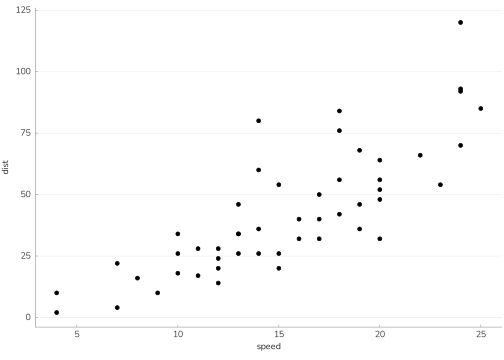
\includegraphics{wp_files/figure-pdf/fig-cars-1.png}

}

\end{figure}%

\chapter{Une section de niveau 1 pour commencer}\label{sec-ledebut}

Lorem ipsum dolor sit amet, consectetur adipiscing elit, sed do eiusmod
tempor incididunt ut labore et dolore magna aliqua. Dolor morbi non arcu
risus quis varius quam quisque.

\section{Section niveau 2}\label{sec-cacontinue}

Faucibus turpis in eu mi bibendum. Etiam tempor orci eu lobortis. Sit
amet consectetur adipiscing elit pellentesque habitant. Quam viverra
orci sagittis eu volutpat odio facilisis mauris sit.

\section{Section niveau 2}\label{sec-encore}

Scelerisque in dictum non consectetur a erat nam at. Elementum facilisis
leo vel fringilla est. Libero enim sed faucibus turpis in eu. Ut lectus
arcu bibendum at varius vel pharetra vel.

\chapter{Une autre section de niveau 1}\label{sec-etencore}

Ultrices neque ornare aenean euismod elementum nisi quis eleifend.
Vivamus arcu felis bibendum ut tristique. Non nisi est sit amet
facilisis magna. Consectetur libero id faucibus nisl tincidunt eget.

\begin{tcolorbox}[enhanced jigsaw, toptitle=1mm, colframe=quarto-callout-tip-color-frame, bottomrule=.15mm, opacitybacktitle=0.6, breakable, colback=white, leftrule=.75mm, arc=.35mm, bottomtitle=1mm, title={les encadrés}, titlerule=0mm, rightrule=.15mm, toprule=.15mm, colbacktitle=quarto-callout-tip-color!10!white, opacityback=0, coltitle=black, left=2mm]

Pour faire un encadré, il faut créer un div .callout-tip. Le titre de
l'encadré est en niveau 2 (\#\#)

En ajoutant l'attribute \texttt{collpase=true}, cet encadré sera replié
en HTML.

En ajoutant l'attribute \texttt{icon=false}, Il n'y a pas d'icone dans
le titre

Il faut utiliser callout-tip, les autres callouts donnent les résultats
standards.

Dans le futur, ce sera plus simple.

\end{tcolorbox}

\section{Section niveau 2}\label{sec-ca-continue}

Amet est placerat in egestas erat imperdiet sed. Non enim praesent
elementum facilisis leo vel fringilla est. Iaculis eu non diam phasellus
vestibulum lorem.

\section{Section niveau 2}\label{sec-encoreetencore}

Eleifend donec pretium vulputate sapien nec sagittis aliquam malesuada
bibendum. Auctor elit sed vulputate mi sit amet.

\begin{figure}

\caption{\label{fig-test}lien entre speed et vitesse}

\centering{

\includegraphics{wp_files/figure-pdf/unnamed-chunk-3-1.png}

Note de lecture\,: Ce format est une alternative

Source\,: une source

}

\end{figure}%

\phantomsection\label{refs}
\begin{CSLReferences}{1}{0}
\bibitem[\citeproctext]{ref-efron1993i}
Efron, Bradley, et Robert J. Tibshirani. 1993. \emph{An Introduction to
the Bootstrap}. Springer US.
\url{https://doi.org/10.1007/978-1-4899-4541-9}.

\end{CSLReferences}



\end{document}
